\documentclass[../Sperimentazione.tex]{subfiles}

\begin{document}

	\section{Interazione utente}
		Per implementare l'interfaccia utente dell'applicazione CLIPS si è cercato di aderire, quanto più fedelmente possibile, al Material Design: specifica promossa da Google per l'implementazione delle interfacce mobile.
		
		La scelta dei colori principali dell'applicazione è stata fatta cercando di minimizzare il numero di tonalità ed aumentare il contrasto, questo garantisce una migliore leggibilità ed un minor affaticamento visivo.

		\subsection{Sezione principale}
			La sezione principale dell'applicazione è stata pensata in modo da fornire all'utente uno sguardo immediato sull'edificio nel quale si trova, a tale scopo sono presenti delle card\g\ che riportano: indirizzo, nome, orari di apertura al pubblico e breve descrizione dell'edificio (figura \ref{fig:HomeCards}). Queste informazioni sono state posizionate all'interno della sezione principale per rendere facile l'accesso alla funzionalità di navigazione. 
			
			\begin{figure} [h]
				\centering
				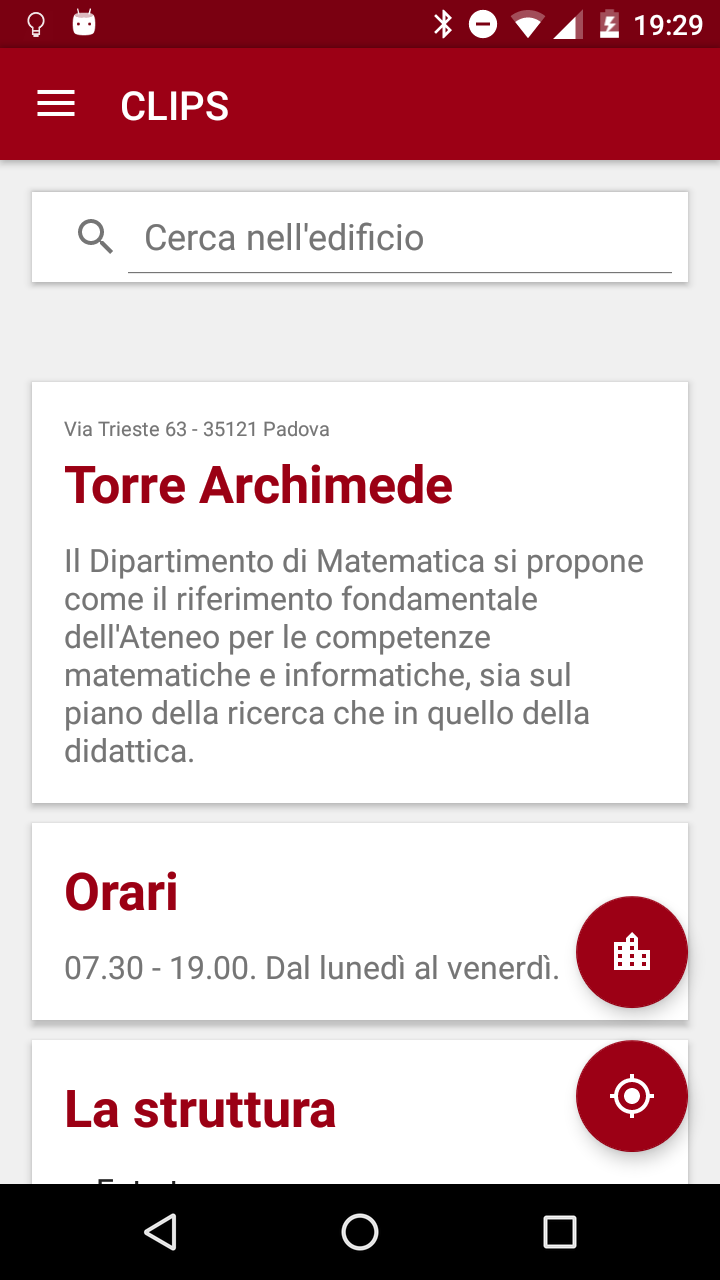
\includegraphics[scale=0.2]{img/home_cards}
				\caption{Sezione principale dell'applicazione}
				\label{fig:HomeCards}
			\end{figure}

	
		La destinazione che si vuole raggiungere può essere indicata secondo due modalità:
		\begin{itemize}
			\item digitandone il nome nell'apposita search box (figura \ref{fig:ListPoiCategory});
			\item scegliendo la categoria della destinazione tra quelle presenti nella card\g\ "La struttura" e, successivamente, scegliendo la destinazione (figura \ref{fig:SearchBox}).
		\end{itemize}
		
			\begin{figure} [h]
				\centering
				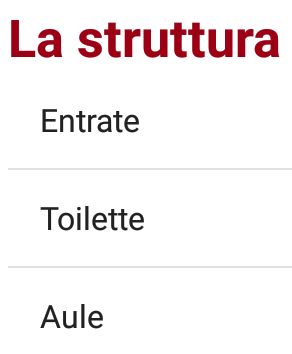
\includegraphics[scale=0.25]{img/list_poi_category}
				\caption{Categorie della struttura mostrate dall'applicazione}
				\label{fig:ListPoiCategory}
			\end{figure}
			
			\begin{figure} [h]
				\centering
				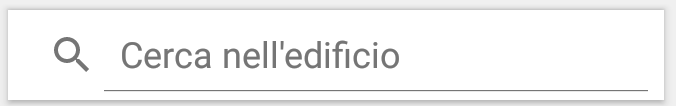
\includegraphics[scale=0.25]{img/searchbox}
				\caption{Casella di ricerca offerta dall'applicazione}
				\label{fig:SearchBox}
			\end{figure}
		
		I diversi tipi di ricerca sono stati pensati per andare incontro alle esigenze di diversi tipi di utenti: mentre la search box può risultare ideale per chi conosce già il nome dell'area che vuole raggiungere, la ricerca per categorie consente all'utente di orientarsi meglio riguardo tra le destinazioni offerte dall'edificio. 
		La search box è dotata di suggerimenti, questo facilita il reperimento della destinazione anche da parte dell'utente che ne ricorda solo parzialmente il nome.

		\subsection{Sezione navigazione}
			Questa sezione ospita le istruzioni utili a raggiungere la destinazione indicata, a partire dalla ROI nel quale ci si trova.
			Le istruzioni vengono fornite sotto forma di lista ordinata: devono essere seguite pedissequamente per raggiungere la destinazione.
			L'istruzione corrente viene evidenziata colorandosi, per essere maggiormente visibile, mentre i passi già compiuti con successo vengono contrassegnati da un check, questo aiuta l'utente a capire a che punto del percorso si trovi in un dato momento.

			Nell'ottica di rendere le istruzioni più facilmente fruibili, sono stati presi alcuni accorgimenti:
			\begin{itemize}
				\item ogni istruzione è associata all'immagine di una freccia che rappresenta la direzione da intraprendere;
				\item ad ogni istruzione è associata la distanza approssimativa da percorrere per raggiungere il prossimo ROI del percorso, tale distanza è espressa in metri nel caso di percorsi piani ed in piani nel caso di scale ed ascensori;
				\item attraverso il tap su un'istruzione è possibile accedere alla versione più dettagliata della stessa, i dettagli aggiuntivi riguardano una descrizione più precisa dei passi da compiere e una serie di foto ritraenti la prossima ROI da raggiungere. Questa sezione è stata pensata in modo che l'utente posso confrontare quello che vede con quello che dovrebbe vedere, così da poter valutare autonomamente se sta seguendo la strada corretta.
			\end{itemize}
			
			\begin{figure} [h]
				\centering
				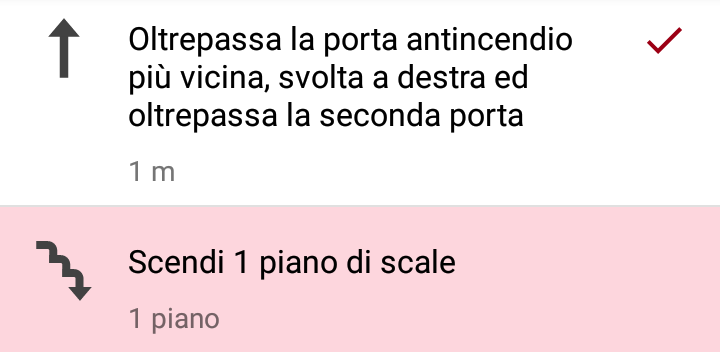
\includegraphics[scale=0.25]{img/list_instruction}
				\caption{Esempio di istruzioni mostrate dall'applicazione}
				\label{fig:ListInstruction}
			\end{figure}

\end{document}